\documentclass[a4paper,10pt]{scrartcl}
\usepackage[a4paper,vmargin={1cm,1cm}%,hmargin={1.5cm,1.5cm}
]{geometry}
\let\raggedsection\centering
\usepackage[english]{babel}
\usepackage{graphicx}
\usepackage{blindtext}
\usepackage{listings}

\lstset{numbers=left, numberstyle=\ttfamily, numbersep=1ex, xleftmargin=0.5cm, %
columns=fixed, basewidth=1.2ex, basicstyle=\ttfamily, showstringspaces=false, aboveskip=\smallskipamount, %
belowskip=\smallskipamount}
\lstset{language=bash}
\renewcommand*{\thelstnumber}{\$}


\begin{document}
\section*{Git - A distributed version control system}
\subsection*{Introduction}
Git is a distributed version control system. Version control system means that it manages a given set of your files and their changes and thus makes it possible to return to any given situation in their history. Distributed means everyone has its own repository. Sharing work with other people means loading their repositories or at least parts of their repositories into your repository.

\subsection*{Install Git on your system}
This may be skipped if you're working on a MPI server because on these Git is already installed.
\begin{itemize}
  \item[\textbf{Linux}] I think you know what to do...
  \item[\textbf{Windows}] You can find under \texttt{http://code.google.com/p/msysgit/downloads/list} the Windows port if Git. Select during the setup "Use Git Bash only", "Use OpenSSH" and "Use Unix style line endings". Of course, you can choose other settings if you know what you do. If Git is set up properly you can start a Git command line in every directory by clicking right on it and choosing "Git Bash Here".
      
  \textit{Remark:} Git is a downright Linux tool and thus the most common way to work with it is to use the command line. However there are some front-ends offering a more Windows like way. TortoiseGit for example integrates seamlessly into your explorer and comes with a complete set of applications to cope with Git. Unfortunately we can't present this software in this article and thus only the plain Git commands will be discussed.
\end{itemize}

\subsection*{Repositories}
\begin{figure}[b]
\centering
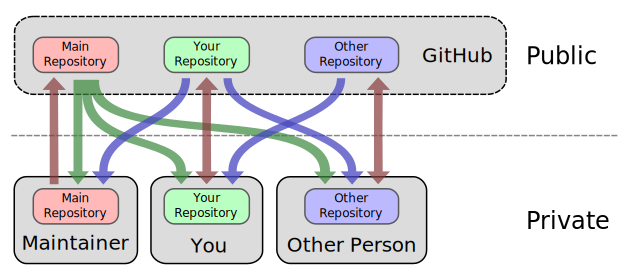
\includegraphics[width=\linewidth]{repos.pdf}
\caption{Repositories}
\label{fig:repos}
\end{figure}
A repository is a database containing all information about the tracked files, their histories, contributing authors and the dates of their contributions. When the directory \texttt{/home/johndoe/gitrepo} is a Git repository it contains a hidden \texttt{.git} directory containing all the above mentioned informations. Besides that a repository usually contains a working tree.
\begin{description} 
 \item[\textbf{Main repository}] The repository containing the official version of the TensorCalculus library. Its (read only) URL is \texttt{git://github.com/waehnert/TensorCalculus.git} and can be used to fetch the newest official version of the package. See Figure~\ref{fig:repos}, green arrows.
  \item[\textbf{Your public repository}] To contribute to the TensorCalculus library you have to create a repository at an public Git hosting site, e.g. GitHub. Since the main repository is already hosted at GitHub it'll be the easiest way to host your public repository also at GitHub. During signing up you get all the nescessary information to get reading and writing access to your account and your public repositories. See Figure~\ref{fig:repos}, red arrow.
%
%After creating an user account you can simply fork from the TensorCalculus main repository by visiting its site at GitHub and pressing the "Fork" button. The public URL to your public repository looks like \texttt{git://github.com/yourname/TensorCalculus.git} and the maintainer of the main repository or other people can pull your contribution from this link. This link only grants reading access. Nobody else than you has writing access to your public repository.
  \item[\textbf{Your private repository}] This repository is a clone of your public repository on your local computer. It's an independet repository and contains the whole history of the project too. You can commit changes, branch and merge these branches as you want. To publish these changes you have to push them into your public respository, see Figure~\ref{fig:repos}, red arrow. If you want to push them into other repositories you can make a pull request to their maintainers, especially to the maintainer of the main repository, see Figure~\ref{fig:repos}, blue arrows.
\end{description}

\subsection*{Important notions}
\begin{itemize}
  \item[\textbf{Repository}] 
  \item[\textbf{Working tree}] The working tree is the content of the directory \texttt{/home/johndoe/gitrepo} \textit{besides} the \texttt{.git} directory. It contains the currently checked out files you can work on to bring in changes and untracked files, which aren't under version control.
  \item[\textbf{Checkout}] If you checkout from your repository you're loading a certain snapshot from your database. All tracked files from this snapshot are loaded to your working tree. Modified but not commited or staged files will be kept and not overriden by a checkout and thus stay modified.
 \item[\textbf{Stage/Index}] Adds the given files to the database but doesn't add a commit object that links these file objects to the history of the project. It can be seen as a kind of a pre-repository where you add all files you'll commit the next time. 
  \item[\textbf{Commit}] As a noun: A object in your database containing a list of pointers to file objects in the database and thus representing a snapshot saved in your repository.\smallskip

    As a verb: Loading all files put into the index into your repository as a new commit.
  \item[\textbf{Branch}] As a noun: A branch is a line in the development history of your repository. Different branches can diverge on a certain point of their histories and merge at a later point.\smallskip

    As a verb: If you're branching you create a new pointer to the head of your current branch. Commits can be made independently to the new and the original branch. From this moment on their histories diverge.
  \item[\textbf{Merge}] To merge one branch B into an other branch A means to merge all changes made in branch B into the branch A. If the two branches differ in the same files in a non trivial manner\footnote{Due to the fact that branching is a very strong feature of Git its merging algorithms can handle fairly complex cases. Nevertheless if for example the same line of a file differs it can't be automatically decided which proceeding will be the right.} Git can't resolve these conflicts and the user has to decide manually how to proceed.
  \item[\textbf{Remote}] A remote is an other repository which history you track, i.e. you push and pull information to and from it to your repository.

  \item[\textbf{Clone}] Clones a repository into a newly created directory, creates remote-tracking branches for each branch in the cloned repository, and creates and checks out an initial branch equal to the cloned repository´s currently active branch.
  \item[\textbf{Push}] Transport the state of your local repository to a remote
  \item[\textbf{Fetch}] Download all file and commit objects from a remote repository into the local repository. This doesn't change your current working directory nor your active branch nor does it any merges. But you can for example create a new branch containing these downloaded objects and finally merge this branch into one of your branches to integrate these changes.
  \item[\textbf{Pull}] The same as fetching followed by merging of each tracked branch of the remote into the corresponding local branch.
  \item[\textbf{Pull request}] If you're ready with some work and want to contribute it back to other repositories you can make a so called pull request. It informs the maintainers of the other repositories that they can pull your new feature from your public repository and merge it into their repositories.
\end{itemize}




\subsection*{Preparation}
%Due to our multiplatform development team this section will be partially divided into a left part for the Linux users and a right part for the Windows users.
\begin{description}
  \item[Fork from the main repository.] This may be skipped if you only want to have a local copy of the main repository and don't want to contribute to the project. Otherwise I recommend to create a public avialable fork on GitHub.
    \begin{enumerate}
      \item Create an own account at GitHub. You'll get all the nescessary information to access its repositories from your local computer.
      \item Go to the site of the main repository at GitHub and press fork to create an fork on GitHub into your account. This repository is your own public repository.
    \end{enumerate}
  \item[Install Git on your system.] 
  \item[Initializing your private repository.] This may be skipped if you already cloned your public repository onto your local computer. 
    Go to your favourite directory and type 
\begin{lstlisting}
git clone git@github.com:yourname/TensorCalculus.git
\end{lstlisting}
    A new directory \texttt{TensorCalculus} will be created containing a clone of the current main repository. A remote called \texttt{origin} which represents your public repository will be automatically set up. To register the official repository as a remote \texttt{upstream} type
\begin{lstlisting}
git remote add upstream git://github.com/waehnert/TensorCalculus.git
\end{lstlisting}
\end{description}
\subsection*{Usual workflow}
\begin{description}
  \item[Update your local repository.] If the main repository was updated it is nescessary to get these newest changes into your local repository.
    To merge the changes blindly you can type
\begin{lstlisting}
git pull upstream master
    \end{lstlisting}
    To check the updates beforhands you have to fetch the newest files
\begin{lstlisting}
git fetch upstream master
\end{lstlisting}
    This doesn't merge the changes into the current branch like \texttt{pull}. To test the changes you have to checkout them into a new branch
\begin{lstlisting}
git checkout -b test upstream/master
\end{lstlisting}
    After thoroughly testing you can merge them into the \texttt{master} branch
\begin{lstlisting}
git checkout master
git merge upstream/master
\end{lstlisting}
    and delete the \texttt{test} branch
\begin{lstlisting}
git branch -d test
\end{lstlisting}
    To delete the changes unmerged you have to write \texttt{-D} instead of \texttt{-d} in the last command.
\end{description}
\end{document}
